\documentclass[border=4pt]{standalone}
\usepackage{tikz}
\usetikzlibrary{arrows.meta,positioning,calc,fit,backgrounds,patterns,shapes.geometric}
\usepackage{amsmath,amssymb}
\usepackage{mathptmx}
\definecolor{lost}{HTML}{C2362D}
\definecolor{kept}{HTML}{17875A}
\definecolor{evid}{HTML}{3056D3}
\definecolor{ink}{HTML}{1D1D1F}
\definecolor{muted}{HTML}{6E6E73}
\tikzset{
  box/.style={draw=ink!70, rounded corners=2pt, align=center, fill=white, inner sep=4pt, font=\footnotesize},
  arr/.style={-{Stealth[length=2mm]}, draw=ink!70, line width=0.6pt},
  grp/.style={draw=muted!60, dashed, rounded corners=4pt, inner sep=7pt},
  lossbox/.style={draw=lost!80, fill=lost!6, text=lost!85!black, rounded corners=2pt, align=left, font=\footnotesize, inner sep=4pt},
  fixbox/.style={draw=kept!80, fill=kept!7, text=kept!65!black, rounded corners=2pt, align=left, font=\footnotesize, inner sep=4pt},
  dec/.style={diamond, aspect=2.2, draw=ink!70, fill=evid!6, align=center, font=\footnotesize, inner sep=1.5pt},
  lbl/.style={font=\footnotesize\bfseries, text=ink},
}

\begin{document}
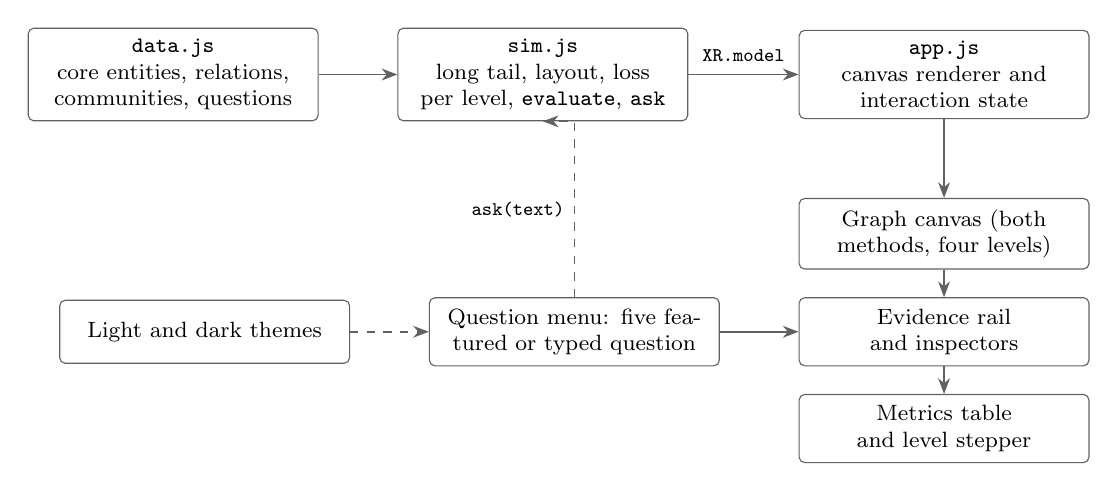
\begin{tikzpicture}[node distance=0.5cm]
\tikzset{m/.style={box, minimum width=3.6cm, minimum height=1.0cm, text width=3.4cm}}
\node[m] (data) {\texttt{data.js}\\core entities, relations, communities, questions};
\node[m, right=1.0cm of data] (sim) {\texttt{sim.js}\\long tail, layout, loss per level, \texttt{evaluate}, \texttt{ask}};
\node[m, right=1.4cm of sim] (app) {\texttt{app.js}\\canvas renderer and interaction state};
\draw[arr] (data) -- (sim); \draw[arr] (sim) -- node[above=1pt, font=\scriptsize] {\texttt{XR.model}} (app);
\node[m, below=1.0cm of app, minimum height=0.8cm] (cv) {Graph canvas (both methods, four levels)};
\node[m, below=0.35cm of cv, minimum height=0.8cm] (rail) {Evidence rail and inspectors};
\node[m, below=0.35cm of rail, minimum height=0.8cm] (met) {Metrics table and level stepper};
\node[m, left=1.0cm of rail, minimum height=0.8cm] (q) {Question menu: five featured or typed question};
\node[m, left=1.0cm of q, minimum height=0.8cm] (th) {Light and dark themes};
\draw[arr] (app) -- (cv); \draw[arr] (cv) -- (rail); \draw[arr] (rail) -- (met);
\draw[arr] (q) -- (rail); \draw[arr, dashed] (q.north) |- node[left, font=\scriptsize, pos=0.25] {\texttt{ask(text)}} (sim.south);
\draw[arr, dashed] (th) -- (q);
\end{tikzpicture}
\end{document}
